%% For double-blind review submission, w/o CCS and ACM Reference (max submission space)
% \documentclass[sigplan,10pt,review,anonymous]{acmart}\settopmatter{printfolios=true,printccs=false,printacmref=false}
\documentclass[sigplan,10pt,review]{acmart}\settopmatter{printfolios=true,printccs=false,printacmref=false}
%% For double-blind review submission, w/ CCS and ACM Reference
%\documentclass[acmsmall,review,anonymous]{acmart}\settopmatter{printfolios=true}
%% For single-blind review submission, w/o CCS and ACM Reference (max submission space)
%\documentclass[acmsmall,review]{acmart}\settopmatter{printfolios=true,printccs=false,printacmref=false}
%% For single-blind review submission, w/ CCS and ACM Reference
%\documentclass[acmsmall,review]{acmart}\settopmatter{printfolios=true}
%% For final camera-ready submission, w/ required CCS and ACM Reference
% \documentclass[acmsmall]{acmart}\settopmatter{}


%% Journal information
%% Supplied to authors by publisher for camera-ready submission;
%% use defaults for review submission.
\acmJournal{PACMPL}
\acmVolume{1}
\acmNumber{CONF} % CONF = POPL or ICFP or OOPSLA
\acmArticle{1}
\acmYear{2018}
\acmMonth{1}
\acmDOI{} % \acmDOI{10.1145/nnnnnnn.nnnnnnn}
\startPage{1}

%% Copyright information
%% Supplied to authors (based on authors' rights management selection;
%% see authors.acm.org) by publisher for camera-ready submission;
%% use 'none' for review submission.
\setcopyright{none}
%\setcopyright{acmcopyright}
%\setcopyright{acmlicensed}
%\setcopyright{rightsretained}
%\copyrightyear{2018}           %% If different from \acmYear

%% Bibliography style
\bibliographystyle{ACM-Reference-Format}
%% Citation style
%% Note: author/year citations are required for papers published as an
%% issue of PACMPL.
% \citestyle{acmauthoryear}   %% For author/year citations


%%%%%%%%%%%%%%%%%%%%%%%%%%%%%%%%%%%%%%%%%%%%%%%%%%%%%%%%%%%%%%%%%%%%%%
%% Note: Authors migrating a paper from PACMPL format to traditional
%% SIGPLAN proceedings format must update the '\documentclass' and
%% topmatter commands above; see 'acmart-sigplanproc-template.tex'.
%%%%%%%%%%%%%%%%%%%%%%%%%%%%%%%%%%%%%%%%%%%%%%%%%%%%%%%%%%%%%%%%%%%%%%


%% Some recommended packages.
\usepackage{booktabs}   %% For formal tables:
                        %% http://ctan.org/pkg/booktabs
\usepackage{subfigure} %% For complex figures with subfigures/subcaptions
                        %% http://ctan.org/pkg/subcaption
\usepackage{xcolor}
\usepackage{listings}
\lstset{
  basicstyle=\fontsize{9}{10}\selectfont\ttfamily,
  numbers=left,
  numberstyle= \tiny,
  keywordstyle= \color{ blue!70},
  commentstyle= \color{red!50!green!50!blue!50},
  frame=single,
  rulesepcolor= \color{ red!20!green!20!blue!20} ,
  escapeinside=``,
  xleftmargin=1.5em,xrightmargin=0em, aboveskip=1em,
  framexleftmargin=2em,
  showstringspaces=false,
  showtabs=false,
  breaklines=true
}
\lstdefinelanguage{Solidity}
{
  morekeywords={contract, mapping, address, uint, private, function, public, if, payable},
  morecomment=[l]{//},
  morestring=[b]"
}


\usepackage{multicol}
\usepackage{multirow}
\usepackage{lipsum}
\usepackage{mathtools}
\usepackage{cuted}
\usepackage{makecell}

\usepackage{amsmath}
\usepackage{extpfeil}
\usepackage{mathpartir}
\usepackage[mathscr]{eucal}

\usepackage{hyperref}
\usepackage{cleveref}
\crefformat{section}{\S#2#1#3} % see manual of cleveref, section 8.2.1
\crefformat{subsection}{\S#2#1#3}
\crefformat{subsubsection}{\S#2#1#3}

\usepackage{algorithm}
\usepackage{algorithmicx}
\usepackage{algpseudocode}
\renewcommand{\algorithmicrequire}{\textbf{Input:}}
\renewcommand{\algorithmicensure}{\textbf{Output:}}

\newcommand{\todo}[1]{\textcolor{red}{[TODO: #1]}}

\begin{document}

%% Title information
\title[Network Fusion through CDRP Model Decomposition and Assembly]{Network Fusion through CDRP Model\\ Decomposition and Assembly}         %% [Short Title] is optional;
%% when present, will be used in
%% header instead of Full Title.
%\titlenote{ }             %% \titlenote is optional;
%% can be repeated if necessary;
%% contents suppressed with 'anonymous'
%\subtitle{Subtitle}                     %% \subtitle is optional
%\subtitlenote{with subtitle note}       %% \subtitlenote is optional;
%% can be repeated if necessary;
%% contents suppressed with 'anonymous'


%% Author information
%% Contents and number of authors suppressed with 'anonymous'.
%% Each author should be introduced by \author, followed by
%% \authornote (optional), \orcid (optional), \affiliation, and
%% \email.
%% An author may have multiple affiliations and/or emails; repeat the
%% appropriate command.
%% Many elements are not rendered, but should be provided for metadata
%% extraction tools.

\author{Zhongye Wang}
% \authornote{Supervised by Qinxiang Cao, Shanghai Jiao Tong University, John Hopcroft Center for Computer Science.}          %% \authornote is optional;
%% can be repeated if necessary
%\orcid{nnnn-nnnn-nnnn-nnnn}             %% \orcid is optional
\affiliation{
	%\position{Position2b}
	%\department{Department2b}             %% \department is recommended
	\institution{Shanghai Jiao Tong University}           %% \institution is required
	%\streetaddress{Street3b Address2b}
	%\city{City2b}
	%\state{State2b}
	%\postcode{Post-Code2b}
	%\country{Country2b}                   %% \country is recommended
}
% \email{wangzhongye1110@sjtu.edu.cn}          %% \email is recommended

\author{Yichen Xie}
% \authornote{Supervised by Qinxiang Cao, Shanghai Jiao Tong University, John Hopcroft Center for Computer Science.}          %% \authornote is optional;
%% can be repeated if necessary
%\orcid{nnnn-nnnn-nnnn-nnnn}             %% \orcid is optional
\affiliation{
	%\position{Position2b}
	%\department{Department2b}             %% \department is recommended
	\institution{Shanghai Jiao Tong University}           %% \institution is required
	%\streetaddress{Street3b Address2b}
	%\city{City2b}
	%\state{State2b}
	%\postcode{Post-Code2b}
	%\country{Country2b}                   %% \country is recommended
}
% \email{}          %% \email is recommended

\author{Xinyu Zhan}
% \authornote{Supervised by Qinxiang Cao, Shanghai Jiao Tong University, John Hopcroft Center for Computer Science.}          %% \authornote is optional;
%% can be repeated if necessary
%\orcid{nnnn-nnnn-nnnn-nnnn}             %% \orcid is optional
\affiliation{
	%\position{Position2b}
	%\department{Department2b}             %% \department is recommended
	\institution{Shanghai Jiao Tong University}           %% \institution is required
	%\streetaddress{Street3b Address2b}
	%\city{City2b}
	%\state{State2b}
	%\postcode{Post-Code2b}
	%\country{Country2b}                   %% \country is recommended
}
% \email{}          %% \email is recommended



%% Abstract
%% Note: \begin{abstract}...\end{abstract} environment must come
%% before \maketitle command
\begin{abstract}
  The abstract \dots
\end{abstract}


%% 2012 ACM Computing Classification System (CSS) concepts
%% Generate at 'http://dl.acm.org/ccs/ccs.cfm'.

%% End of generated code


%% Keywords
%% comma separated list
\keywords{}  %% \keywords are mandatory in final camera-ready submission


%% \maketitle
%% Note: \maketitle command must come after title commands, author
%% commands, abstract environment, Computing Classification System
%% environment and commands, and keywords command.
\maketitle

\section{Introduction}
\label{sec:intro}
The introduction \dots

\begin{figure}[h]
    \centering
    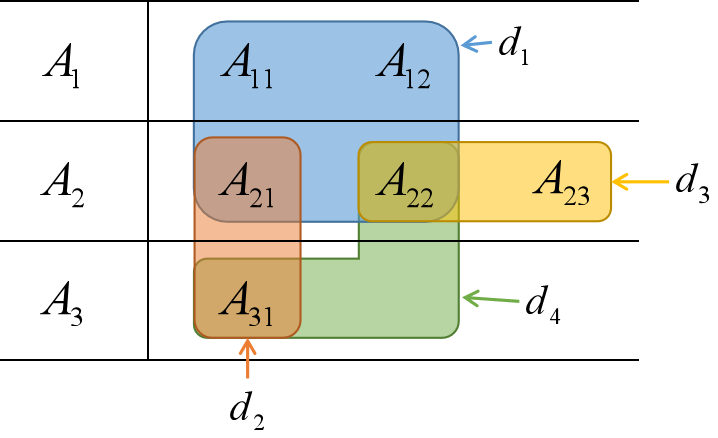
\includegraphics[width=0.75\linewidth]{fig/formulation_example.png}
    \caption{An Example Assembly Problem}
    \label{fig:assemble-example-venn}
\end{figure}

\Cref{fig:assemble-example-venn} shows an example of the assembly problem of our interest.
The original dataset contains 3 classes $A_1, A_2$, and $A_3$, and we are able to decompose each into some subclasses, e.g., $A_1$ is decomposed into two subclasses of samples $A_{11}$ and $A_{12}$.
There are 4 binary classifiers, each determines whether a sample belongs to the union of some subclasses marked with boxes, e.g., $d_1$ determines whether a sample belongs to the union of $\{A_{11}, A_{12}, A_{21}, A_{22}\}$.
We can use classifiers $d_1, d_2, d_3$ and set operations for the classification task:
\begin{itemize}
	\item $d_1 - (d_2 + d_3)$ determines samples belong to $A_1$;
	\item $d_1 \cdot d_2 + d_3$ determines samples belong to $A_2$;
	\item $d_2 - d_1$ determines samples belong to $A_3$.
\end{itemize}
For the partial classification task of class $A_3$, it suffices to use only $d_2$ and $d_4$ and their intersection $d_2 \cdot d_4$ to determine samples in $A_3$.

\subsection{Our Work}

\section{The General Assembly Framework}
\label{sec:assembly}
In this section, we give the general framework to assemble multiple classifiers into one that performs complex classification tasks.
The classification task only need to cover a given set of labels, and we do not need to distinguish the remaining dummy classes.
We also propose an heuristic search algorithm to find a feasible solution to the assembly problem.

We only consider the general case of such assembly in this section, while we specialize the assembly problem w.r.t. input composed of CDRP models in \cref{sec:cdrp}.
The assembly problem can be easily extended to general classifier input, but we only discuss the case for binary classifier input for simplicity.

\subsection{The Assembly Problem}
\label{sec:assemble-problem}
We first formulate the problem by defining the input of an assembly problem and the output it requires.

The input have the following components:
\begin{itemize}
	\item $L$ class labels, denoted $\{l_j\}$
	\item $N$ subclasses in total \begin{itemize}
		\item $M$ target subclasses, denoted $\mathcal{A} = \{A_i\}$
		\item $N-M$ dummy subclasses, denoted $\bar{\mathcal{A}} = \{A_i\}$
	\end{itemize}
	\item $g(A_i) := l_j$ the partial map from $A_i$ to class label $l_j$
	\item $K$ classifiers, denoted $\mathcal{D} = \{d_j\}$
	\item $f(A_i, d_j) := 0, 1$ the classifier certificate function that $A_i$ is classified positive in classifier $d_j$
	\item $score(d_j)$ the performance score of classifier $d_j$
	\item $k$ the maximum number of classifier to use
\end{itemize}

The original dataset consists of $L$ classes with different labels.
Some prior knowledge allows us to decompose the dataset into $N$ subclasses of samples.
A subclass is the unit sample group we will consider in the assembly problem, and for a subclass to be \textit{consistent}, we assume all samples in a subclass have the sample label given by the partial map $g$.
Since we are only interested in a subset of labels, we group all $M$ target subclasses having these labels into $\mathcal{A}$
The rest $N-M$ subclasses are dummy ones.

We are given $K$ binary classifiers with domains of the entire dataset.
All samples in a subclass $A_i$ should be assigned the same 0-1 label by a classifier $d_j$, which is determined by the certificate function $f$.
To extend the assembly problem to general classifier inputs, we only need to change the certificate function $f$ for classifiers to allow return values from a set of multiple symbols.
The cardinality of $f$'s range should be $n$ for an $n$-classifier assembly problem.
For example, a ternary classifier assembly problem needs the certificate function to produce three possible symbols, i.e., $|range(f)| = 3$.

For each classifier, we also know its performance score, which could be its accuracy, its model complexity, or both.
There is a constraint for a problem instance that we can only use up to $k$ classifiers to assemble the final classifier.

The solution to the problem instance should contain:
\begin{itemize}
	\item $D \subset \mathcal{D}$ a set of $m$ classifiers \textit{distinguishing} all $M$ target subclasses s.t. $m < k$
	\item $score(D)$ the overall performance of the classifier set
\end{itemize}

\todo{The overal performance score.}

We define the concept of \textit{distinguishing} as follows.
\begin{definition}
	A set of classifiers covers $M$ target subclasses iff. given any sample, the joint classifier can determine whether it \textit{solely} belongs to \begin{enumerate}
		\item a subset (with consistent labels) of the $M$ target subclasses, or,
		\item the rest dummy subclasses $\bar{\mathcal{A}}$.
	\end{enumerate}
\end{definition}
In other word, the classifier should uniquely determine whether a sample have which of the target labels or the dummy label.

We start with analyzing the intractability of the problem.
\begin{theorem}
	The assembly problem is an NP problem.
\end{theorem}
\begin{proof}
We prove the theorem by giving a polynomial algorithm for the certificate problem.

Given a certificate $D \subset \mathcal{D}$, we encode each subclass with a binary string $s$ of length $k$, where the $j$-th element for the $i$ subclass is $f(A_i, d_j)$ ($d_j \in D$).
This step takes $O(Nk) = O(NK)$ time.
The algorithm returns $yes$ iff. \begin{enumerate}
	\item No two subclasses in $\mathcal{A}$ share the same encoding but have different labels, and,
	\item No subclass in $\mathcal{A}$ shares the same encoding with any subclass in $\bar{\mathcal{A}}$.
\end{enumerate}
Otherwise, it returns $no$.
This step takes $O(N)$ if we use hash table to record the occurrence of encoded strings.

% \begin{algorithm}[h]
% 	\caption{}
% 	\begin{algorithmic}
% 		\Require A assembly problem instance $k$; a certificate $D \subset \mathcal{D}$.
% 		\Ensure Whether problem instance $k$ is solvable.
% 		\State initialize a hash table $H$ with default value -1;
% 		\For{$i = 1, \cdots, N$}
% 			\For{$d_j \in D$}
% 				\State $s_{i,j} \leftarrow f(A_i, d_j)$;
% 			\EndFor
% 			\If{$H[s_i]$ != $g(A_i)$}
% 				\State \Return $no$
% 			\ElsIf{$H[s_i]$ == -1}
% 				\State a
% 			\EndIf
% 		\EndFor
% 	\end{algorithmic}
% \end{algorithm}

We then show the algorithm returns $yes$ iff. $D$ is a certificate to the problem.
\begin{enumerate}
	\item[$\Rightarrow$:]
	The encoding for each target subclass is different from that of another subclass having different labels, meaning the classifier set can distinguish them from subclasses with other labels, and it is then clear that $D$ covers all target subclasses.
	\item[$\Leftarrow$:]
	Assume the algorithm returns $no$, then
	\begin{enumerate}
		\item Two subclasses with different labels share the same encoding, i.e., the classifier set cannot determine which label to assign for both subclasses, which violates the first condition of the \textit{distinguishing};
		\item Some target subclass (with meaningful label) share the same encoding with some dummy subclasses.
		The classifier set cannot determine whether samples of the target subclass belong to the dummy class or not, which violates the second condition.
	\end{enumerate}
	Therefor, $D$ is not a certificate to the problem.
\end{enumerate}
As a result, the problem instance $k$ is solvable iff. there exists a $D$ with size $k$ such that the algorithm returns $yes$.
By definition, the problem is an NP problem.
\end{proof}

\Cref{tab:assemble-example-encoding} shows the encoding mentioned in the certificate algorithm for the intro example in \cref{fig:assemble-example-venn}.
If we only use the encoding from $d_1, d_2, d_3$, we find no two subclasses with different labels share the same encoding, and therefore certify the correctness of the feasible solution proposed before.
For the partial classification task for $A_3$, using two bits from $d_2, d_4$ already provides distinguishable encoding for $A_{31}$ and the remaining dummy classes.

% \linespread{1.1}
\begin{figure}[h]
	\begin{tabular}{|c|c|cccc|}
	\cline{1-6}
	\multicolumn{2}{|c|}{} & $d_1$ & $d_2$ & $d_3$ & $d_4$ \\ \cline{1-6}
	\multirow{2}{*}{$A_1$} & $A_{11}$ & 1 & 0 & 0 & 0 \\ \cline{2-6}
	 & $A_{12}$ & 1 & 0 & 0 & 0 \\ \cline{1-6}
	\multirow{3}{*}{$A_2$} & $A_{21}$ & 1 & 1 & 0 & 0 \\ \cline{2-6}
	 & $A_{22}$ & 1 & 0 & 1 & 1 \\ \cline{2-6}
	 & $A_{23}$ & 0 & 0 & 1 & 0 \\ \cline{1-6}
	$A_3$ & $A_{31}$ & 0 & 1 & 0 & 1 \\ \cline{1-6}
	\end{tabular}
	\caption{Encoding for the Intro Example}
	\label{fig:assemble-example-encoding}
\end{figure}
% \linespread{1.0}

\subsection{The Heuristic Search Algorithm}
\label{sec:assembly-algorithm}
Based on the encoding method, we propose a search algorithm based on greedy heuristics in \cref{tab:heuristic-search} for finding a feasible solution to the problem instance with constraint $k$.

\begin{algorithm}[h]
	\caption{The General Algorithm}
	\label{tab:heuristic-search}
	\begin{algorithmic}[1]
		\Require The inputs to the assembly problem;
		\Ensure $D$, a classifier set satisfying constraints, or $\emptyset$ if not feasible.
		\State $Q \gets \emptyset$; \Comment A priority queue, the last element $h$ is the key
		\Function{Expand}{$D$} \Comment $D$, the classifier set
			\For{$d \in \mathcal{D} - D$}
				\State Calculate the encoding $C$ using $D \cup \{d\}$;
				\State Calculate the entropy $h$ for $C$;
				\State $Q \gets Q \cup \{(D \cup \{d\}, C, h)\}$;
			\EndFor
		\EndFunction
		\Function{HeuristicSearch}{}
			\State $\Call{Expand}{\emptyset}$;
			\While{$Q \neq \emptyset$}
				\State $(D, C, h) \gets Pop(Q)$;
				\If{$e_0 == 0$}
					\State \Return $D$;
				\EndIf
				\If{|D| < k}
					\State $\Call{Expand}{D}$;
				\EndIf
			\EndWhile
			\State \Return $\emptyset$;
		\EndFunction
	\end{algorithmic}
\end{algorithm}

The search is guided by the residual entropy \eqref{eq:entropy} of target subclasses and dummy subclasses.
\begin{equation}
	H(C) = \sum_{c \in C} p(c)H(c) = \sum_{c \in C} p(c)\sum_{l \in \mathcal{L}'} p(c, l)\log\frac{1}{p(c, l)}
	\label{eq:entropy}
\end{equation}
where $p(c)$ is the probability for encoding $c$ to occur, and $p(c, l)$ is the probability of a sample having encoding $c$ and label $l$.
Note that the label ranges over $\mathcal{L}'$, the set of target labels and one dummy label, and all labels that are not target is defined to be equal to the dummy one.
In each search iteration, the algorithm will choose the classifier set that minimizes the entropy greedily, so that the search could possibly to end with minimum search depth.

\todo{Analysis}

\section{Model Assembly based on CDRP Decomposition and Clustering}
\label{sec:cdrp}
In \cref{sec:assembly}, we have formalized the problem and proposed a general algorithm searching for a feasible solution to a search problem instance.
In this section, we want to instantiate the assembly problem in a concrete setting.
To do so, we need to find an efficient way to generate the input to the problem.
More specifically, we need to find an initial set of binary classifiers with following constrains.
\begin{itemize}
	\item The initial set should guarantee at least one feasible solution for some $k$.
	\item There should exist overlapping subclasses among classifiers to allow multiple choices, i.e., allow removing of redundant feature extractors.
	\item We can not train a large set of binary classifiers from scratch, because it takes too many prior knowledge and time to get an initial set that have feasible solution with the space for improvements.
\end{itemize}



\paragraph{Remark.} We do not need to provide the subclasses in the input, because they can be derived from the initial set of classifiers.
Given encodings under the initial classifier set, samples share the same encoding can be considered as a subclass, and there is no need to further split those subclasses.
For example, in the intro example in \cref{fig:assemble-example-venn}, there is no need to distinguish $A_{11}$ and $A_{12}$ and we can group them as a single subclass.

To satisfy the above constraints, we follow the previous work of Wang \textit{et al.} \cite{wang2018interpret} to use critical data routing path (CDRP) for generating the input.
CDRP clustering allow us to decompose a large network model into several disjoint small ones.
To have overlapping classifiers, we decompose two different networks on the same dataset and fine tuning the CDRP models into binary classifiers.
We use image classification task on CIFAR-100 and VGG16 of type C and D for demonstration.

\subsection{CDRP Decomposition and Clustering}
Guideline:
\begin{itemize}
	\item How to train gates, the functionality of the gates, how to interpret gate weight (lambda) feature of samples (similar to original paper)
	\item How to get decomposed classifiers: clustering
	\item Why clustered CDRP models might work (PCA visualization demonstration) (not performance analysis, inference experiments later)
	\item Why fine tuning the clustered CDRP model into binary classifiers, and how we fine tune them
\end{itemize}

Critical Data Routing Path is a method to find a path containing critical nodes, whose removal causes great preformance setback, from an existing trained model. We introduce CDRP to decomposite one existing pretrained model from selecting representing CDRPs in a given dataset.

\paragraph{CDRP extraction}

From the original model, we introduce a scalar control gate to every output channel of one layer, with nonnegative and sparse value. They will be multiplied to the layer’s output channelwise, resulting in the routing nodes. The nodes that are not suppressed, or have control gate weight greater zero, will be linked together to compose the routing paths. Then finding the critical data routing path can be reduced to optimize the weights of the control gates.

Critical data routing path is extracted through optimizaition of control gates values. We freeze the weights of the model, and for each sample we follow the procedure of Distillation Guided Routing (\cref{alg:dgr}) \cite{wang2018interpret} to get the gate values. The gate values can be concatenated into one single vector as representation of that sample. As the original paper \cite{wang2018interpret} states, these gate values encode patterns inside the input images, e.g. tinca in horizontal positions or squat positions will have different encodings.

\begin{algorithm}
	\caption{Distillation Guided Routing, introduced in paper \cite{wang2018interpret}}
	\label{alg:dgr}
	\begin{algorithmic}[1]
		\Require Input image $\boldsymbol{x}$, pretrained network $f_\theta(\cdot)$, control gates $\boldsymbol{\Lambda}$ initialized with 1, balanced parameter $\gamma$. Max iterations $T$, SGD optimizer
		\Ensure identified CDRPs representation $\boldsymbol{v}$
		\State original prediction class $i \gets \arg\max f_\theta(\boldsymbol{x})$
		\For{$t \gets 1$ to $T$}
			\State compute loss $cur\_loss$: $$\mathcal{L}\left(f_\theta(\boldsymbol{x}), f_\theta(\boldsymbol{x}; \boldsymbol{\Lambda})\right) + \gamma \sum_k |\boldsymbol{\lambda}_k|_1$$
			\State compute control gates gradients $\boldsymbol{\Lambda}$: $$\frac{\partial Loss}{\partial \boldsymbol{\Lambda}} = \frac{\partial \mathcal{L}}{\partial \boldsymbol{\Lambda}} + \gamma \times \mathrm{sign}(\boldsymbol{\Lambda})$$
			\State update $\boldsymbol{\Lambda}$ by SGD optimzier and clip $\boldsymbol{\Lambda}$ to be nonnegative
			\State new prediction class $j \gets \arg\max f_\theta(\boldsymbol{x};\boldsymbol{\Lambda})$
			\If{$i=j$} \Comment keep the prediction same
				\If{$cur\_loss$ is minimun}
					\State $\boldsymbol{v} \gets \mathrm{concatenate}(\boldsymbol{\Lambda})$
				\EndIf
			\EndIf
		\EndFor		
	\end{algorithmic}
\end{algorithm}

\paragraph{CDRP clustering}

The fact that CDRP as encoding of samples directly leads to the idea that decompoisite one large model into several smaller models, each of which processing one pattern of input data. Once the gate vectors of all samples is obtained, we use k-means clusterng to cluster these vectors to gather samples sharing similar patterns together.

The visualization of clustering results is presented in \cref{fig:vgg-cluster-pca}.

\begin{figure}[!htp]
	\centering
	\subfigure[Result of VGG-16(C)] {
		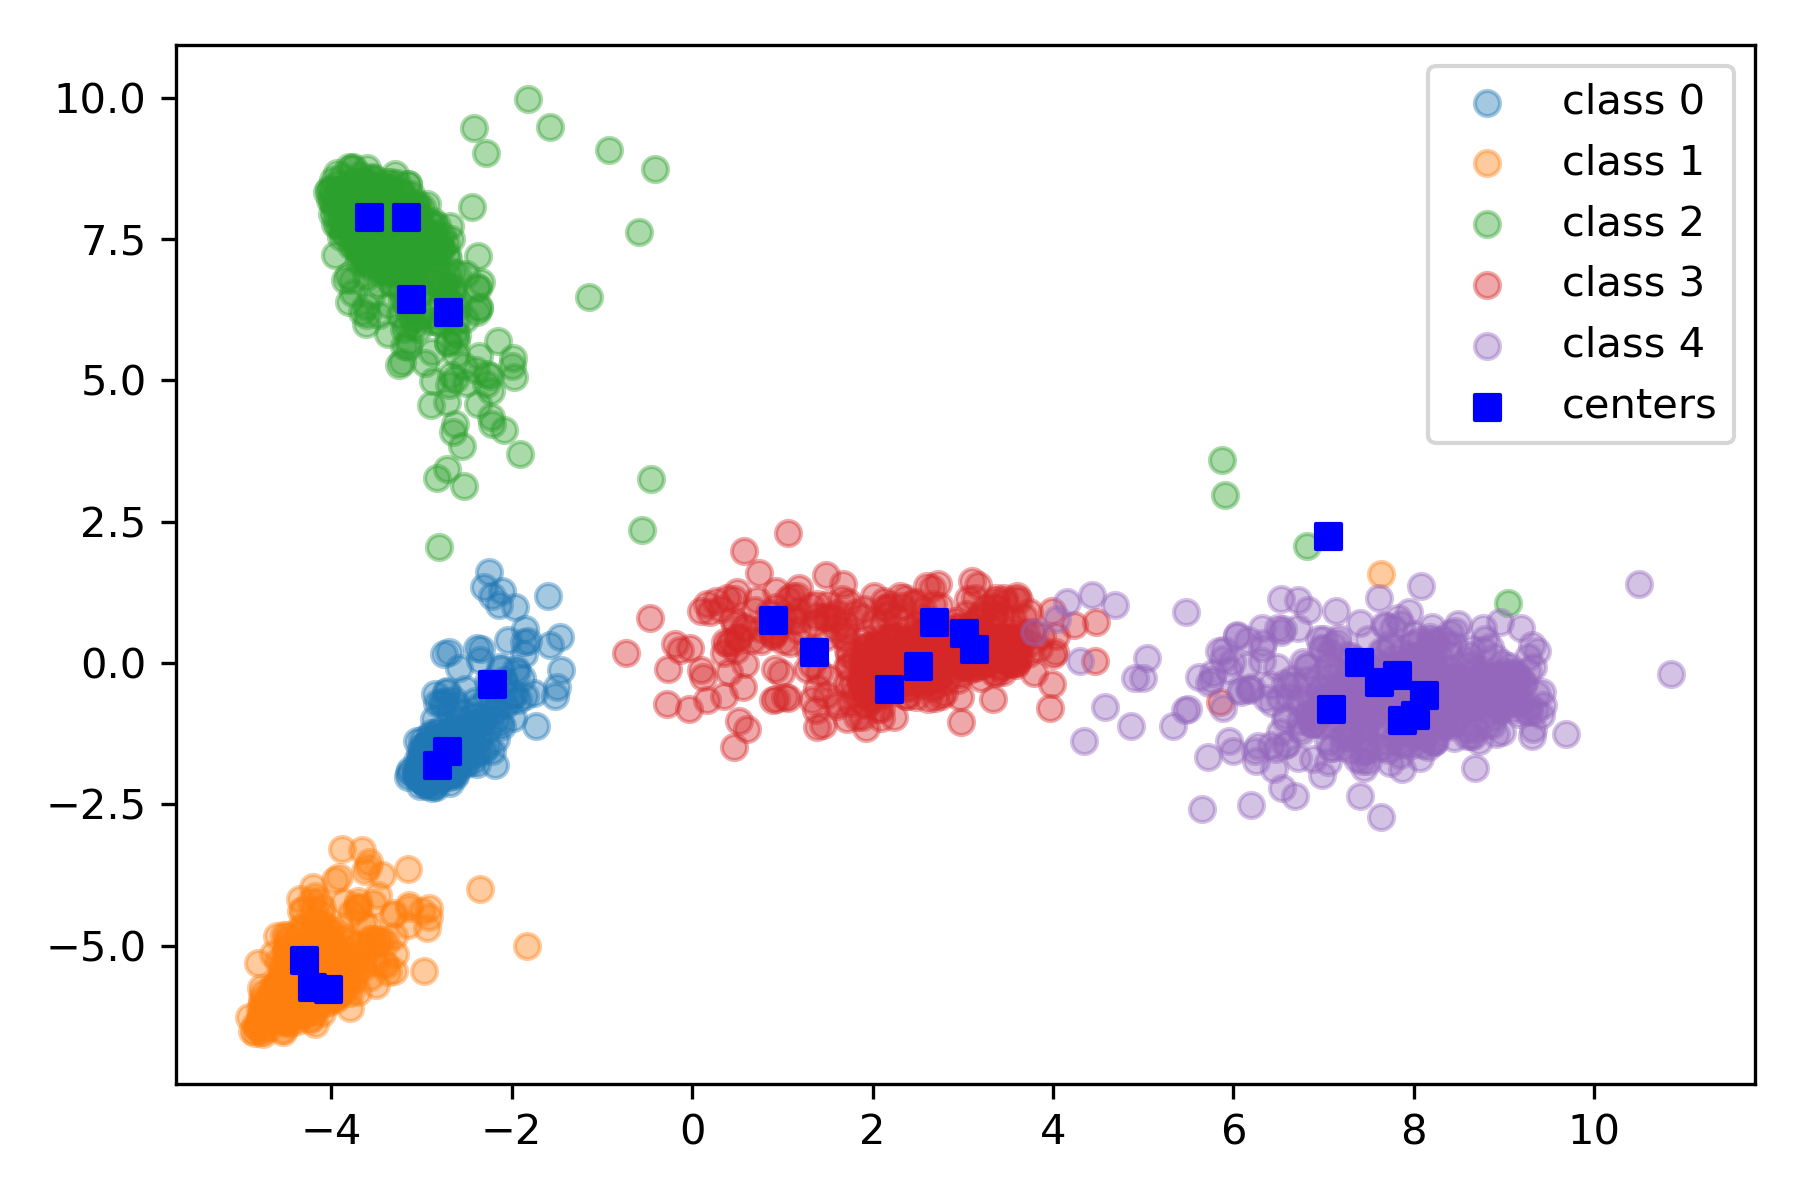
\includegraphics[width=\linewidth]{fig/vgg16c-cluster.png}
        \label{fig:vgg16c-cluster}
	}
	\subfigure[Result of VGG-19(D)] {
		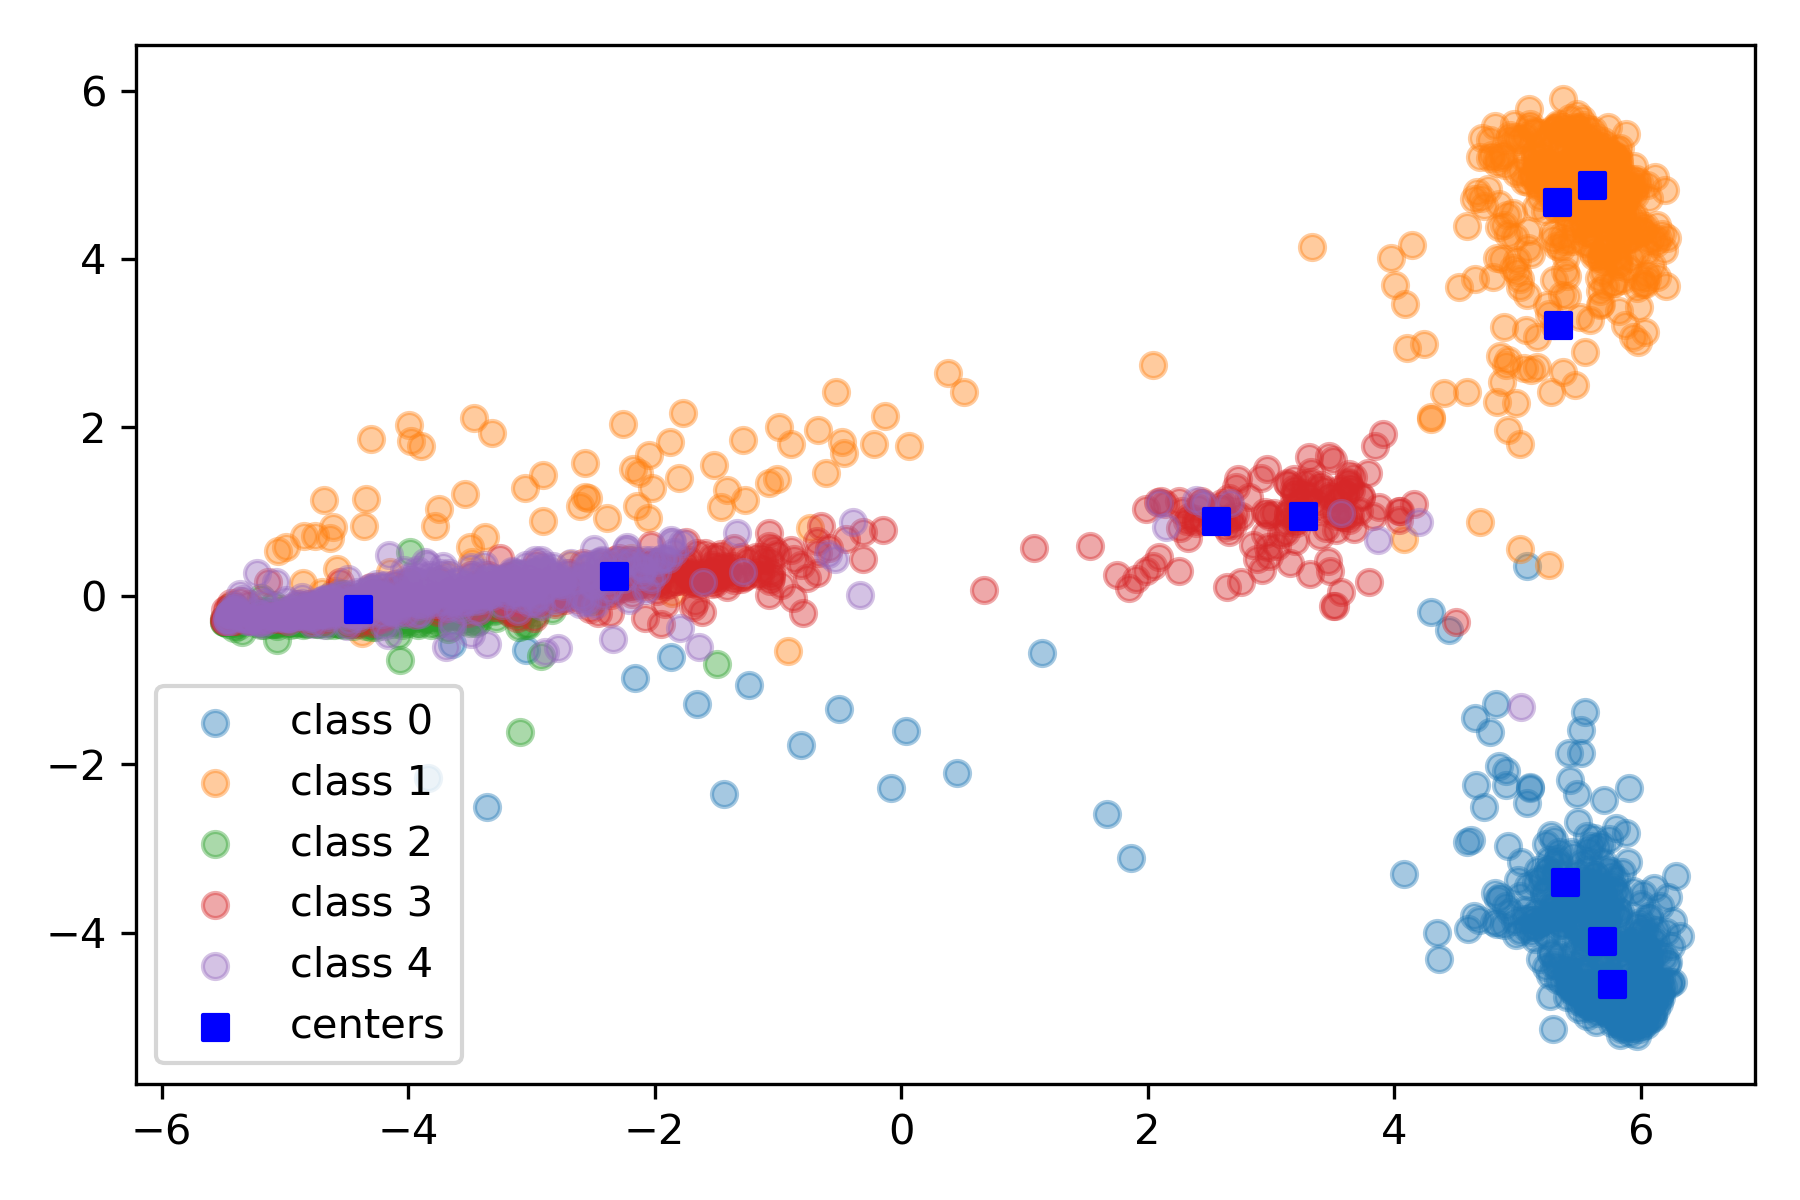
\includegraphics[width=\linewidth]{fig/vgg16d-cluster.png}
        \label{fig:vgg16d-cluster}
    }
    \caption{Visualization of clustering results. The axes are the first two components of of PCA results on all extracted gate vectors. The figure in the top is the result of VGG-16 (type C) trained on cifar-100 dataset, and the one below is the result of VGG-16 (type D) fine-tuned on cifar-100 initialized with pretrained weights on ImageNet. Different colors represent different class labels in cifar-100 dataset, and the cluster centers are denoted as blue squares.}
    \label{fig:vgg-cluster-pca}
\end{figure}

From the visualization result, it can be observed that the clustering can distinguish samples of difference class lables, i.e. samples in one cluster are not prone to have different class labels. Besides, gate vectors extracted on the same data by different models differs.

The results shows we can derive a good basis of binary classifers through these clusters. First, the good mapping from cluster to class label means we can use these binary classifiers to construct subclasses mentioned in the beginning of this section. The fact that gate vectors from different models varies will prevent the trival case that cluster one-to-one map to class label, leading to substantial reduction on number of model parameters.

\paragraph{Model pruning and fine tuning}

We use methods introduced in paper \cite{LiDongYue} to prune the model according to gate vector of cluster centers (\cref{alg:prune}).

\begin{algorithm}
	\caption{Model Pruning of clusters}
	\label{alg:prune}
	\begin{algorithmic}[1]
		\Require input images of one given cluster $TargetImages$, pretrained network $f_\theta(\cdot)$, $prune\_ratio$
		\Ensure Pruned neural network $f_{\theta'}(\cdot)$
		\State $Paths = \{\}$
		\For{each given training image $\boldsymbol{x}$ in $TargetImages$}
			\State $Path_{\boldsymbol{x}} = \mathrm{DistillationGuidedRouting}(\boldsymbol{x}, f_\theta(\cdot))$
			\State $Paths.add(Path_{\boldsymbol{x}})$
		\EndFor		
		\State compute cluster-wise critical data routing path $SumPath$ via merging $Paths$, resulting gate vector $\boldsymbol{\Lambda} = [\boldsymbol{\lambda}_k]$
		\For{$\boldsymbol{\lambda}_k$ in the $k$-th convolution layers}
			\State sort all $\lambda$s in $\boldsymbol{\lambda}_k$ decreasingly and discard the channels in the last within range of $prune\_ration$
		\EndFor
	\end{algorithmic}
\end{algorithm}

Afterwards we modify the network architecture of fully connected layers to form a binary classifer $g_{\theta'}(\cdot)$. The reason to do this includes:
\begin{itemize}
	\item It has less parameters than 100-class classifers.
	\item It is easier to train, i.e. easier to have higher accuarcy.
	\item Weights of convolution layers in the orginal model could be reused. We just need to finetune the model without running long sessions to train from scratch.
\end{itemize} 

We finetune this model with samples having positive labels in the clusterwhich is used to prune the model, and all other samples having negative labels. 

%\todo{metion CIFAR-5}
\subsection{CDRP Model Assembly}
Based on the results of CDRP decomposition in VGG16-C and VGG16-D, we determine subclasses for CIFAR-5	\footnote{CIFAR-5 is a shorthand refering to samples having the first 5 class labels in CIFAR-100.} and their relationship to the CDRP clusters by encoding samples using all CDRP models.
Instead of using Venn diagram like the intro example in \cref{fig:assemble-example-venn}, we use the network diagram in \cref{fig:network-venn} to represent the relationship between subclasses and clusters.

\begin{figure}[h]
	\centering
	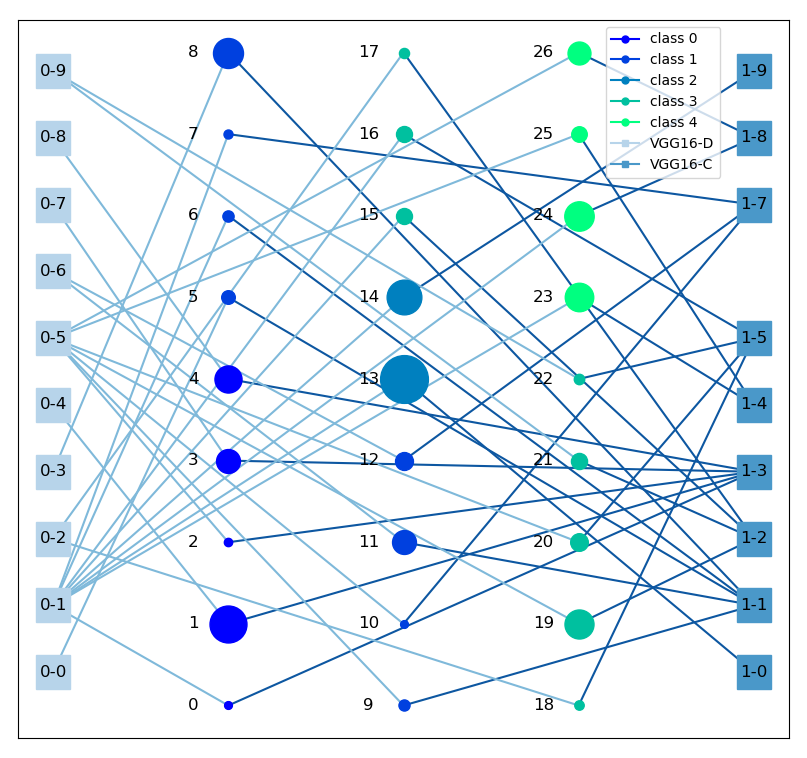
\includegraphics[width=\linewidth]{fig/network_venn.png}
	\caption{Network Venn Diagram for CIFAR-5}
	\label{fig:network-venn}
\end{figure}

The cluster nodes (boxes) on the right side of the figure represent CDRP clusters in VGG16-C, and those on the left side represent clusters in VGG16-D.
The subclass nodes (circles) in the middle represent subclasses, the size of which indicate the number of samples belonging to the subclass and the color of which indicate the label assigned to it.
A subclass node is connected with a cluster node iff. the subclass is a subset of the cluster.

Since we decompose two networks into two sets of internally disjoint clusters, each subclass will fall into exactly two clusters from separate models.
In other word, the encoding for a subclass is a two-hot encoding.
\todo{This means that the assembly problem can be solved with more efficient algorithms.}

\section{Experiments}
\subsection{Verifying CDRP Models of VGGNets trained on CIFAR-100}
In this section, we perform K-Means on the CDRP control gates of each sample. For each cluster, we get a binary-classifier to determine whether the test sample should be in the cluster. Then, we fine tune each classifier in the CIFAR-100 dataset.

\paragraph{Clusters.} For VGGNet, we generate $1.5$ clusters per class.
Then, we get $14$ clusters from $5$ classes, among which $7$ clusters are from VGG16-C and $7$ clusters from VGG16-D. 

The sample distribution of each cluster is shown in Figure~\ref{fig:vgg-cluster}.

\begin{figure}[!htp]
    \centering
\subfigure[Clusters from VGG-C]{
    \begin{minipage}[t]{1\linewidth}
        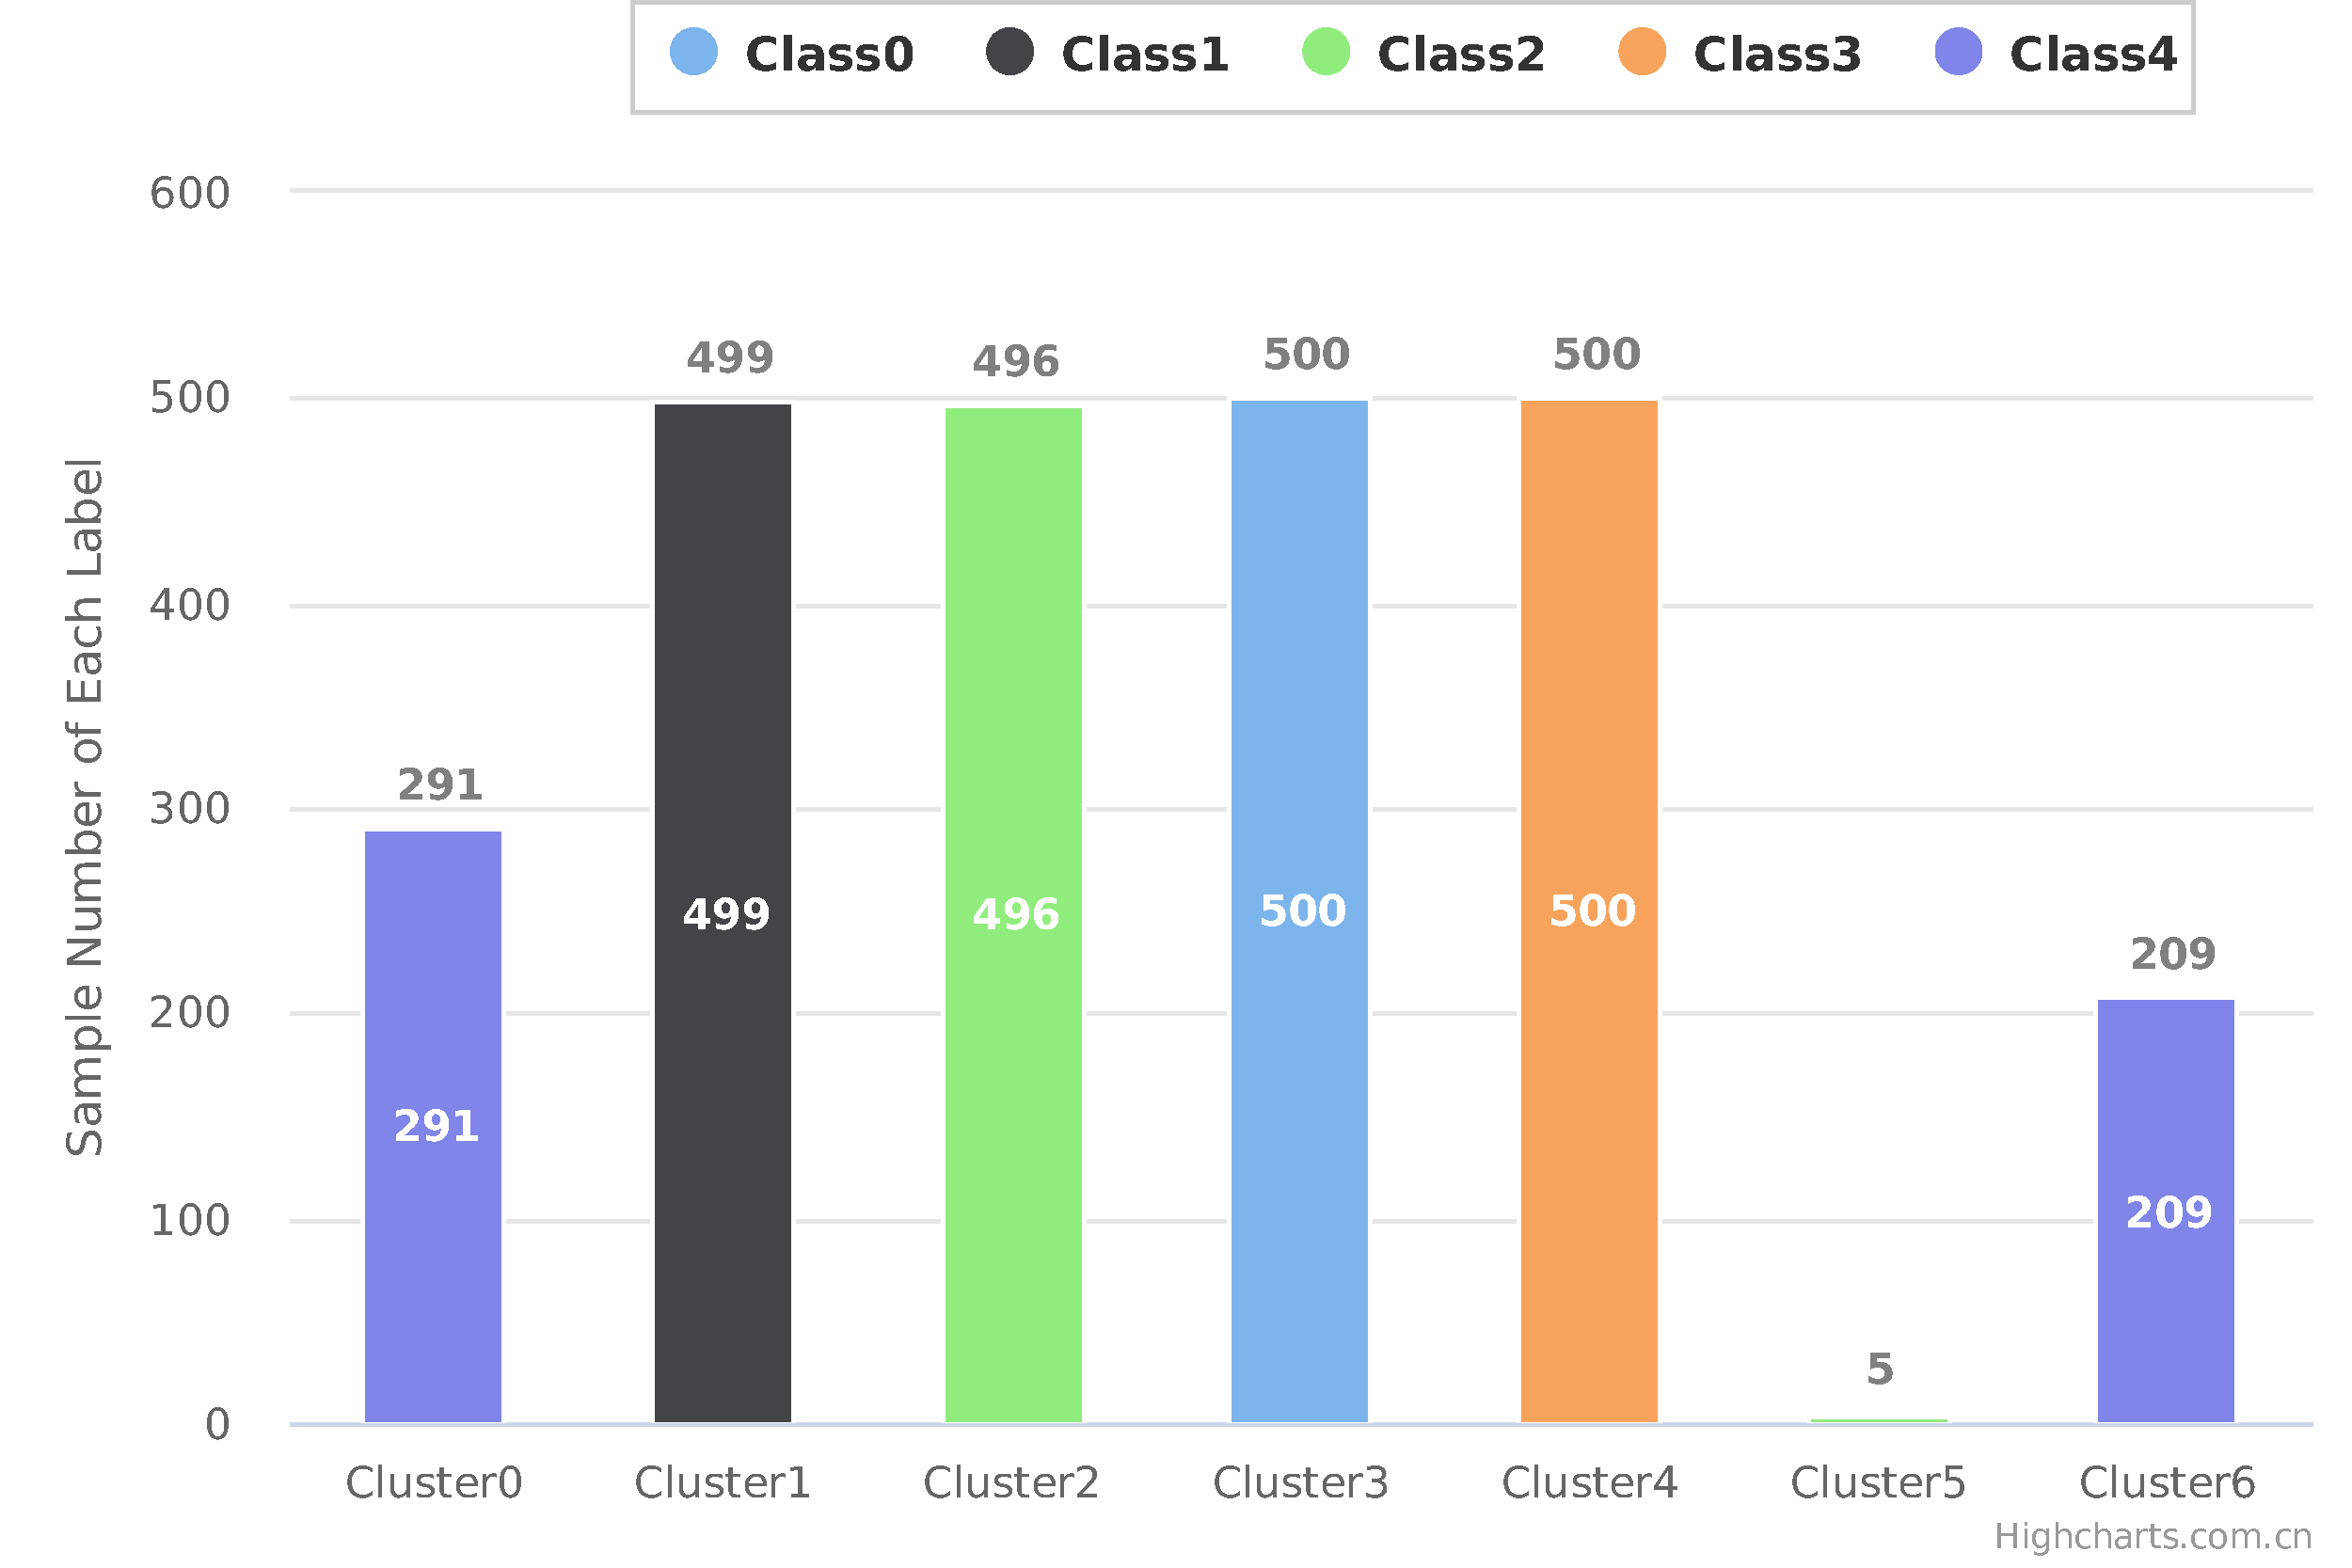
\includegraphics[height=1.5in,width=2.8in]{fig/chart1.pdf}
        \label{fig:net2a}
    \end{minipage}
}

    %\vfill
\subfigure[Clusters from VGG-D]{
    \begin{minipage}[t]{1\linewidth}
        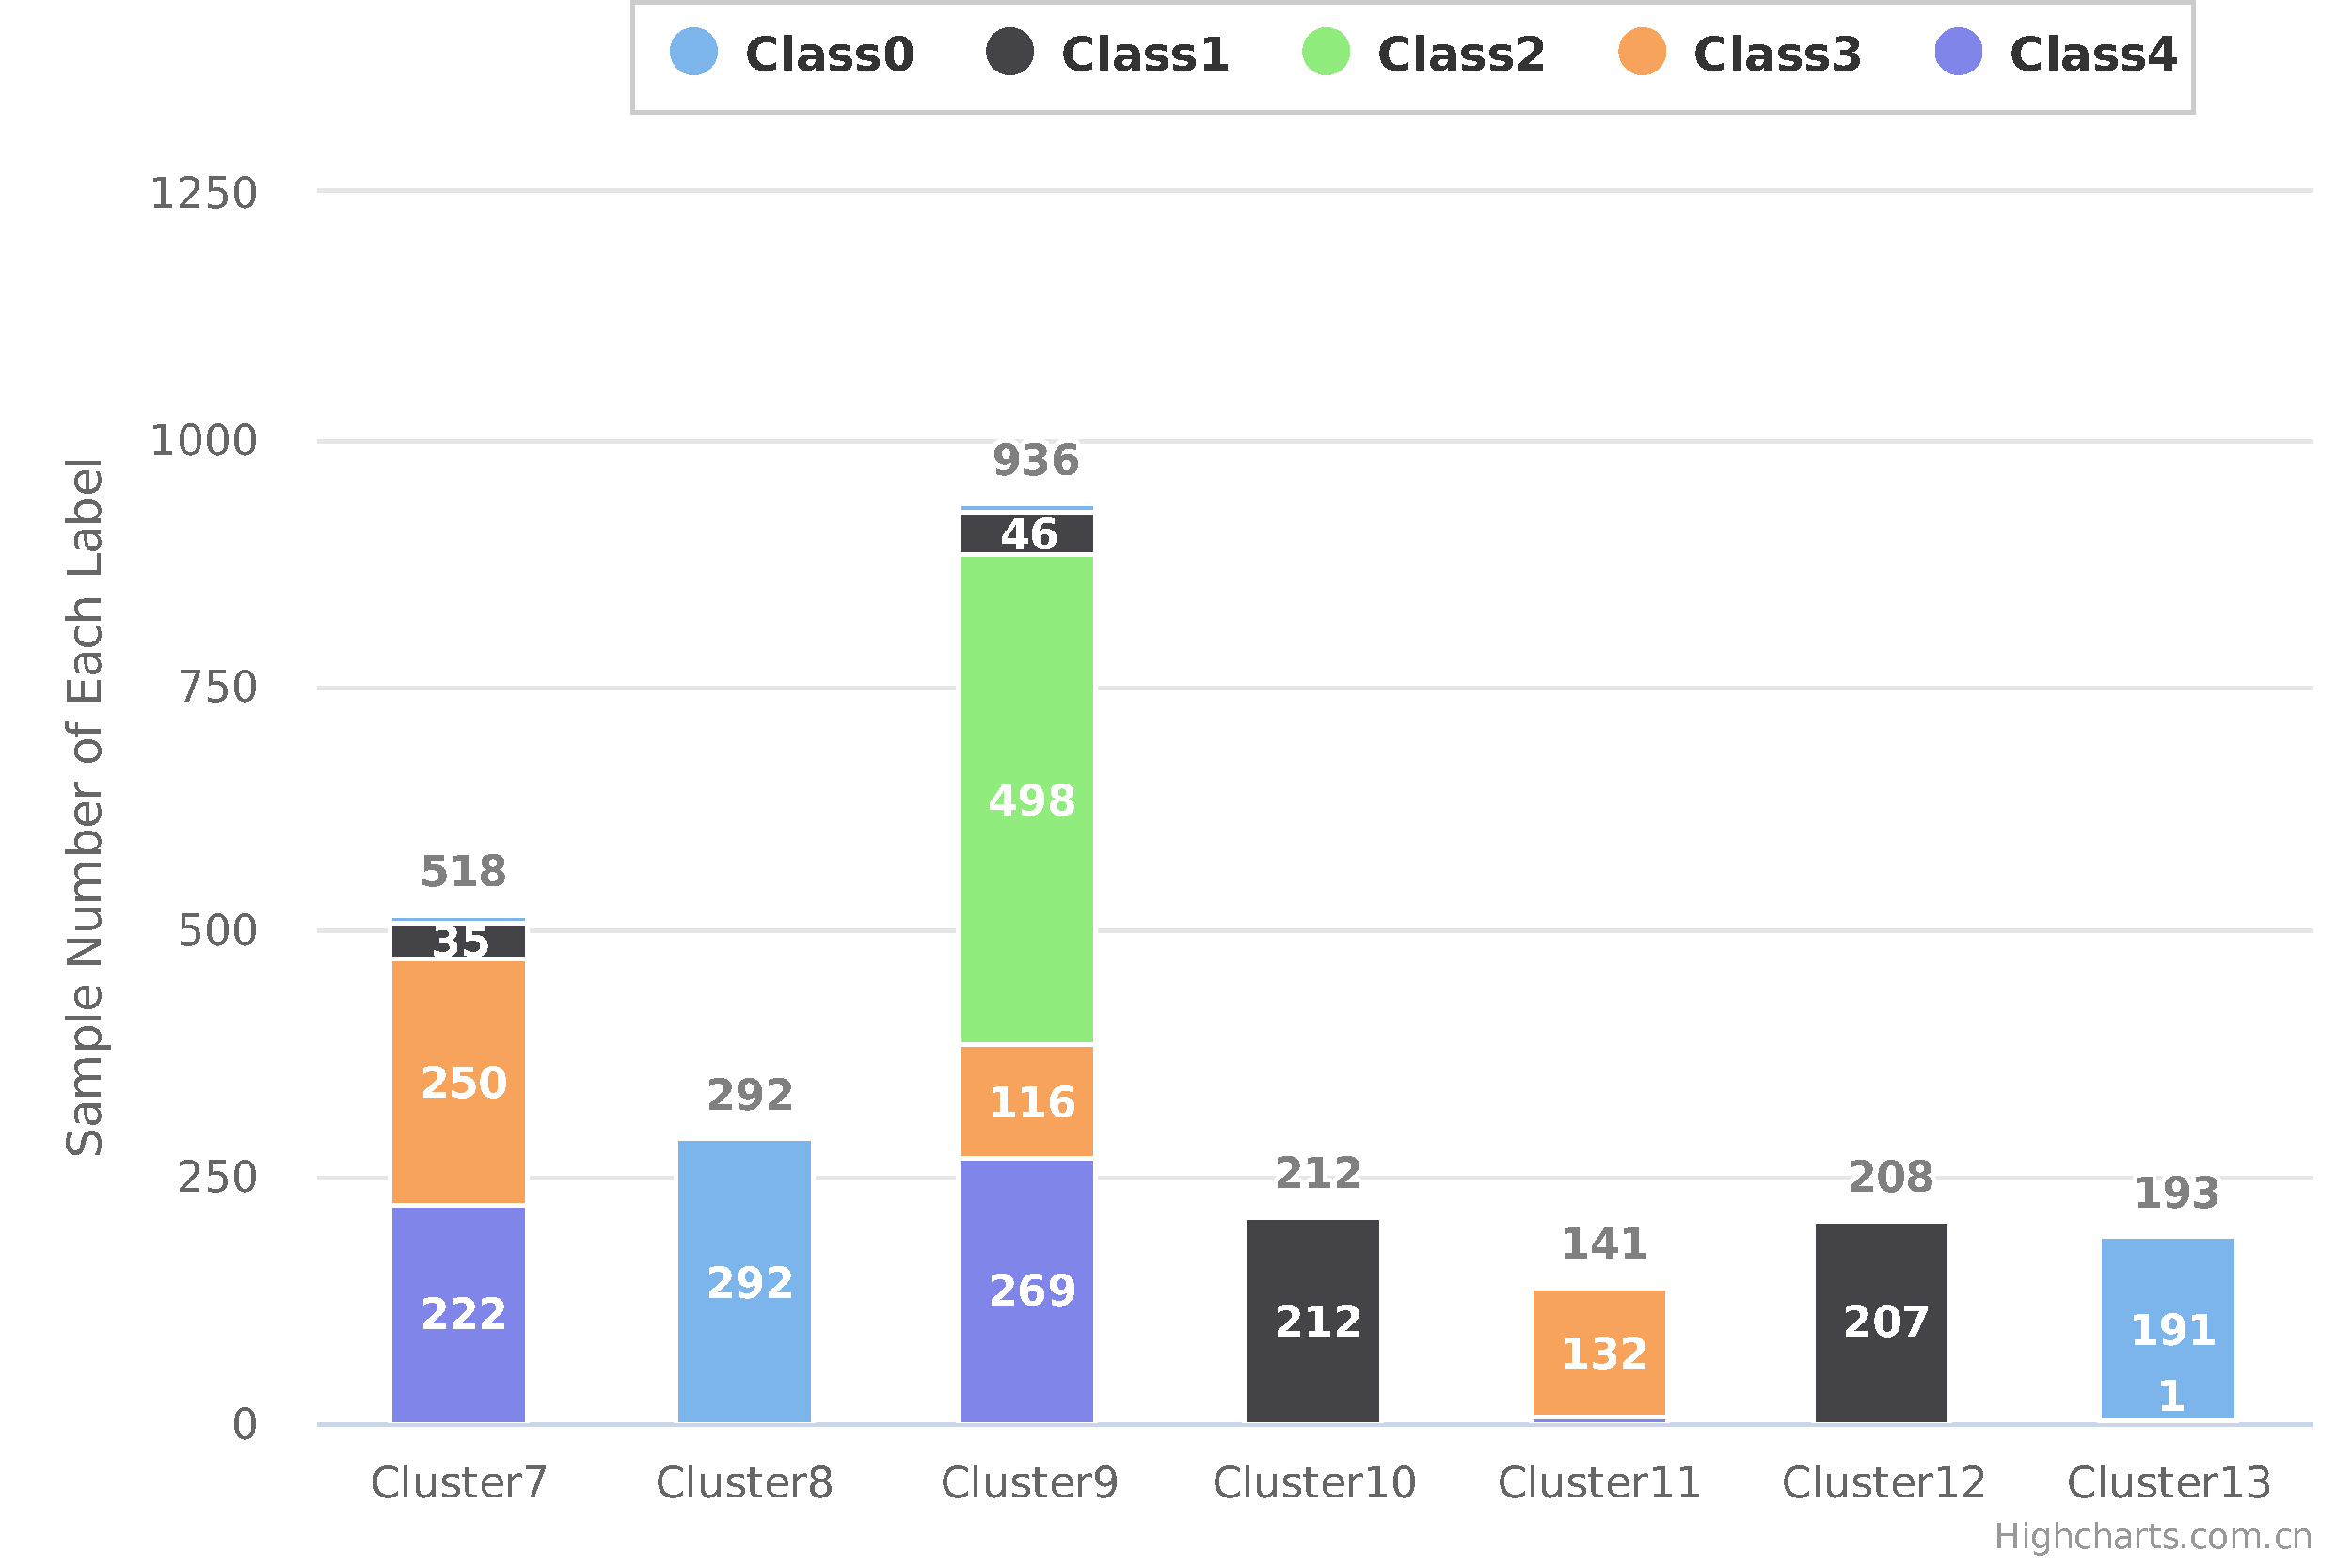
\includegraphics[height=1.5in,width=2.8in]{fig/chart2.pdf}
        \label{fig:net2b}
    \end{minipage}
}
    \caption{Sample Distribution of Clusters from Different Types of VGGNets}
    \label{fig:vgg-cluster}

\end{figure}

From \cref{fig:vgg-cluster}, a cluster from VGG-C typically consists of samples from a single class, which is consistent with the result shown in \cref{fig:vgg-cluster-pca}. 
By contrast, a cluster from VGG-D may contain samples with different labels.

We notice that some clusters only contain extremely few samples such as Cluster-5 so we won't take these clusters into account when choosing classifiers.

\paragraph{Classifiers.} Except some too small ones, we consider one cluster as a classifer. Each classifier judges whether the test sample should in the corresponding cluster. 
From \cref{fig:vgg-cluster}, we determine the possibile labels of samples in each cluster as is shown in \cref{tab:cluster_label}. 

\begin{table}[h]
	\caption{Corresponding Class Labels of Each Cluster}
	\label{tab:cluster_label}
	\begin{tabular}{|c|c|c|}
	\hline
	\multirow{2}{*}{Classifier} &\multicolumn{2}{|c|}{Possible Class Labels}\\
	\cline{2-3}
	& In (0) & Not in (1)\\
	\hline
	classifier-0,6 & 4 & 0,1,2,3,4,5\\
	classifier-1 & 1 & 0,2,3,4,5\\
	classifier-2 & 2 & 0,1,3,4,5\\
	classifier-3 & 0 & 1,2,3,4,5\\
	classifier-4 & 3 & 0,1,2,4,5\\
	classifier-7 & 3,4 & 0,1,2,3,4,5\\ 
	classifier-9 & 2,3,4 & 0,1,5\\ 
	classifier-8,13 & 0 & 1,2,3,4,5\\
	classifier-10,12 & 1 & 0,1,2,3,4,5\\
	classifier-11 & 3 & 0,1,2,3,4,5\\
	\hline
	\end{tabular}
\end{table}

Since we want to get binary-classifiers, we slightly change the original VGGNet architecture in output dimension of the last Fully-Connected Layer from $100$ to $2$. 
We also prune the original full VGGNet in the guide of CDRP with a prune ratio $pr$ i.e. if $pr=0.9$, $90\%$ of channels in all layers are pruned. 
As a result, each classifer only has $10\%$ parameters of the original full network.

\paragraph{Finetune.} The classifiers we get above cannot achieve any meaningful results because they tend to classifiy all test samples not in the cluster and the weights of the last layer is initialized randomly.
We implement finetune on these classifers to make the results more meaningful and accurate. 
Since the negative samples are greatly more than positive ones in the dataset, we need to implement some strategies to balance them i.e. in each iteration we ensure the ratio of positive and negative samples is about $1:1$ in the batch.

We train each classifer with $1500$ iterations with a batch size $200$. 
The learning rate is $0.1$ for the first $1200$ iterations and $0.01$ for the remaining $300$ iterations. 
We only train the pruned model i.e. weights of the pruned channels will remain zero.
With a prune ratio $pr\leq0.9$, most of the classifers can reach an accuracy more than 80\% after finetune, which is much higher than the overall accuracy of the original full network.
 

 
\subsection{Fusing VGGNets for Specific Tasks through CDRP Assembly}
In this section, we implement the heuristic search in \cref{tab:heuristic-search} to fuse the classifiers. According to the 0/1 result of each classifer, we can get an unique encoding for each sample, which corresponds to a unqiue label so that we can determine the class of each test sample.

\paragraph{Fusion}We implement \cref{tab:heuristic-search} to fuse the classifiers since we want to finish a specific task of classifying among five classes, we set a upper bound of the number of classifiers $k=4$. 
After we select these classifiers with this \cref{tab:heuristic-search}, different results of each classifier ($0$ and $1$ represent the sample is or isn't in the cluster respectively) correspond to a unique label.
In our implementation, the algorithm choose four classifiers: 3,4,1,2 in order. 
The accuracy of the four classifiers with different prune ratio is shown in \cref{tab:classifer-accuracy}.The test set has also been balanced to make the number of positive and negative samples nearly $1:1$. 


\begin{table}[h]

    \caption{Accuracy of Chosen Binary-Classifiers}
    \label{tab:classifer-accuracy}
	\begin{tabular}{|c|c|c|c|c|}
	\hline
	Classifier ID & 3 & 4 & 1 & 2 \\
	\hline
	\begin{tabular}{c}Accuracy\\pr=0.95\end{tabular} & 62.3\% & 82.3\% & 83.5\% & 67.0\%\\
	\hline
	\begin{tabular}{c}Accuracy\\pr=0.9\end{tabular} & 96.0\% & 86.0\% & 91.5\% & 87.0\%\\
	\hline
	\begin{tabular}{c}Accuracy\\pr=0.8\end{tabular} & 97.5\% & 80.5\% & 94.5\% & 89.5\%\\
	\hline
	\end{tabular}
\end{table}

\paragraph{Verifying Result.}By combining the 0/1-results of the four classifiers, we can determine the class label unqiuely of one test sample.
For example, if the result of classifer-3 is $0$ whether results of others are all $1$s, the encoding will be $0111$ and we can determine the sample is in class $0$. 

Actually, we can determine the class uniquely with the prefix of encodings. 
For instance, if the result of classifer-3 is $0$, we don't need to take other classifers into consideration since the only class $0$ is possible in cluster-3 according to \cref{tab:cluster_label}

The corresponding encoding of each class label is shown in \cref{tab:encoding-and-accuarcy}. 
We can determine the class label with this encoding, the accuracy of which is also shown in \cref{tab:encoding-and-accuarcy}. 


\begin{table}[h]

    \caption{Encoding and Accuracy of Each Class Label}
    \label{tab:encoding-and-accuarcy}
	\begin{tabular}{|c|c|c|c|c|c|c|}
	\hline

	Class ID & 0 & 1 & 2 & 3 & 4 & Overall \\
	\hline
	Encoding &0 & 110 & 1110 &10 & 1111 & -\\
	\hline
	\begin{tabular}{c}Accuracy\\pr=0.95\end{tabular} & 100\% & 30.0\% & 11.0\% & 28.0\% & 7.0\% & 34.4\%\\

	\hline
	\begin{tabular}{c}Accuracy\\pr=0.9\end{tabular} & 92.0\% & 93.0\% & 58.0\% & 85.0\% & 67.0\% & 79.0\%\\
	\hline
	\begin{tabular}{c}Accuracy\\pr=0.8\end{tabular} & 95.0\% & 91.0\% & 76.0\% & 78.0\% & 76.0\% & 83.2\%\\

	\hline

	\end{tabular}
\end{table}

From \cref{tab:encoding-and-accuarcy}, we find the overall accuracy is quite high if prune ratio $pr\leq0.9$ while the accuracy drops dramatically when $pr=0.95$ since we prune too much channels or even destroy the connectivity of the network. 
When it comes to the trade-off between parameter number and overall accuracy, it is suitable to set prune ratio $pr=0.9$.

Compared to the accuracy of original full model in these $5$ classes ($70.57\%$), our classifier not only achieve higher precision but also improve the efficiency. 
When $pr=0.9$, we can infer with the $4$ binary-classifiers in parallel instead of applying the original network, which can save about $90\%$ computing consumption on a single device as well as improve the accuracy.

\section{Related Work}
The related work \dots

\section{Conclusion}
The conclusion \dots

% Acknowledgments

% Bibliography
% \bibliographystyle{acm}
% \bibliographystyle{unsrt}
\bibliography{../full_list.bib}


%% Appendix
%\appendix
%\section{Appendix}

%Text of appendix \ldots

\end{document}